\documentclass[11pt, english]{article}              
        \usepackage{geometry}
                \geometry{                          
                        a4paper,total={210mm,297mm},
                        tmargin=40.8mm,
                        bmargin=40.8mm,
                        lmargin=32.6mm,        
                        rmargin=32.6mm,                     
                }                                     
                                
	\renewcommand{\theparagraph}{\thesubsubsection.\arabic{paragraph}}

        \usepackage{titlesec}         
                \titleformat{\section}
                        {\normalfont\fontsize{18}{16}\bfseries}{\thesection}{0.5em}{}
                \titleformat{\subsection}
                        {\normalfont\fontsize{14}{16}\bfseries}{\thesubsection}{1em}{}
                \titleformat{\subsubsection} 
                        {\normalfont\fontsize{11}{16}\bfseries}{\thesubsubsection}{1em}{}
 		\titleformat{\paragraph} 
                        {\normalfont\fontsize{11}{16}\bfseries}{\theparagraph}{1em}{}

        \usepackage{longtable}                                                  
        \usepackage{multirow}                                                   
                             
        \usepackage[labelfont=bf,textfont=bf,font=small,skip=8pt]{caption}
                               
        \setlength{\parindent}{0pt}                                 
        \renewcommand{\baselinestretch}{1.25}      
        \usepackage{setspace}                             
                                                                        
        \usepackage{amsmath}                                                    
        \usepackage{amssymb}                                      
                             
        \usepackage{graphicx}                  
                               
        \usepackage{float}                                                

	\usepackage{tikz}
                                                  
\begin{document}                               
                                              
\pagenumbering{gobble}       
                       
        \title{\textsc{EC315 Topics in Microeconomics with Cross-Section Econometrics\\ Coursework Summary}}
        \author{\textsc{Lewis Britton}}
        \date{\textsc{Academic Year 2019/2020}}
        \maketitle

\newpage
                         
\pagenumbering{roman} 
                                                                           
        \renewcommand{\contentsname}{Table of Contents}
                                       
        \tableofcontents

\newpage 

\pagenumbering{arabic}

\section{Exam Summary}

	\subsection{Cost-Benefit Analysis Summary}

	\begin{enumerate}
	\setlength\itemsep{0cm}
		\item Purpose
		\item Alternatives
		\item Who
		\item C/B Impacts
		\item Lifetime Impacts
		\item Monetize:
		\begin{itemize}
			\item \textit{Social Cost}: harm done to living organisms
			\item \textit{Revealed/Stated Preference}: willingness to pay or willingness to accept
			\begin{itemize}
				\item Revealed: shown in behaviour
				\item Stated: questionnaires etc.
			\end{itemize}
			\item \textit{Time}:
			\begin{itemize}
				\item Work vs leisure using wage rate 
				\item Travel time; how much people are willing to trade-off
			\end{itemize}
			\item \textit{Lives}: life expectancy, pay, age, risks taken
			\item \textit{Natural Resources}: AONBs, surveys, investment, regulation
		\end{itemize}
		\item PV Discounts
		\begin{itemize}
			\item Social discount rate
			\item Intergenerational (more than 50 years)
		\end{itemize}
		\item NPV of Alternatives
		\item Sensitivity Analysis
		\item Recommend
	\end{enumerate}

	\newpage

	\subsection{Program \& Policy Evaluation Summary}

	\begin{center}Cause $\longrightarrow$ Intermediaries $\longrightarrow$ Effect\end{center}

	\begin{enumerate}
	\setlength\itemsep{0cm}
		\item Omitted Variable Bias
		\begin{itemize}
			\item Selection Bias: e.g. grades, income, area of ogigin
			\item Selection Bias 2: e.g. effort, determination, stamina
		\end{itemize}
		\item Randomized Control Trial
		\begin{itemize}
			\item Unbiased Estimator: $\bar{x}\longrightarrow\bar{\mu}$ (LLN)
			\item Unbiased Estimator: randomization
			\item $\sigma^2$: ``how much of the result is due to chance?''
			\item t-tests: causal effect; $(\bar{Y}^T-\bar{Y}^C)$
		\end{itemize}
		\item Regression
		\begin{itemize}
			\item Dummy Variables: causal variable / group
			\item Instrumental Variables: omitted variables ($\alpha$ corr. w/ $\varepsilon$)
		\end{itemize}
	\end{enumerate}

	\newpage

	\subsection{Crime \& Punishment Summary}

	\begin{enumerate}
	\setlength\itemsep{0cm}
		\item Supply: $\pi_t=\pi_i-c_i-w_i-p_i(f_i)$
		\begin{itemize}
			\item $i$ = Individual
			\item $\pi_t$ = Net Total Payoff of Crime
			\item $\pi_i$ = Expected Payoff Per Offense (Minus Costs)
			\item $c_i$ = Cost Incurred if Caught
			\item $w_i$ = Wage Rate From Non-Criminal Work
			\item $p_i$ = Probability of Aprehension \& Conviction
			\item $f_i$ = Punishment in Convicted
		\end{itemize}
		\item Normal Distribution
		\begin{itemize}
			\item Req. $\uparrow\pi,\ \uparrow\delta,\ [\bar{x}\rightarrow\mathrm{(Right\ of\ Mean)}]$
			\item Req. $\downarrow\pi,\ \downarrow\delta,\ [\leftarrow\bar{x}\mathrm{(Left\ of\ Mean)}]$
			\item Morals, enjoyment, risk, some demand for significantly higher payoffs etc. effect decision
		\end{itemize}
		\item Demand: $e_if(v_r,v_l);q$
		\begin{itemize}
			\item $e_i$ = Expenditure on Protection
			\item $v_r$ = Risk of Victimization
			\item $v_l$ = Loss of Victim
			\item $q$ = Total Crime
		\end{itemize}
		\item Derivatives
		\begin{itemize}
			\item $\frac{\partial e_i}{\partial v_i}>0$: Risk $\uparrow$, Expenditure $\uparrow$
			\item $\frac{\partial c_i}{\partial e_i}<0$: Expenditure $\uparrow$, Cost $\uparrow$
			\item $\frac{\partial\pi_i}{\partial c_i}<0$: Cost $\uparrow$, Payoff $\downarrow$
		\end{itemize}
		\item Supply / Demand
		\begin{itemize}
			\item 
\includegraphics[width=5cm,height=4cm]{EC315-IMG/1.png}
			\item $ss$ = Supply of Crime
			\item $dd$ = Initial Demand
			\item $\pi\pi$ = Demand After Government Intervention ($T$)
			\item $MC$ of Catching Last Criminal $>$ $MB$ [$\leftarrow\pi^*,\ q^*$]
			\item $MC$ of Catching Last Criminal $<$ $MB$ [$\pi^*,\ q^*\rightarrow$]
		\end{itemize}
	\end{enumerate}

	\newpage

	\subsection{Exam Arithmetic Summary}

	\begin{enumerate}
	\setlength\itemsep{0cm}
		\item $\pi_A=x_Ap_A(x_A+x_B)-x_A$
		\item $J=\pi_A+\pi_B;\ \frac{\partial J}{\partial x_A}=\frac{\partial\pi_A}{\partial x_A}+\frac{\partial\pi_B}{\partial x_B}$
		\item Externalities: $\frac{\partial\pi_A}{\partial x_B}$
		\begin{itemize}
			\item $>0$: Positive: ``you do $\uparrow$, my $\pi$ $\uparrow$''
			\item $<0$: Negative: ``you do $\uparrow$, my $\pi$ $\downarrow$''
		\end{itemize}
		\item Strategic Nature: $\frac{\frac{\partial\pi_A}{\partial x_A}}{\partial x_B}$
		\begin{itemize}
			\item $>0$: Complements: ``you do $\uparrow$, I do $\uparrow$''
			\item $<0$: Substitutes: ``you do $\uparrow$, I do $\downarrow$''
		\end{itemize}
		\item Grim Trigger Strategy
		\begin{itemize}
			\item 40, 50, 30
			\item $\frac{40}{(1-\delta)}\ge50+\frac{30\delta}{(1-\delta)}$
			\item $40\ge50-50\delta+30\delta$
			\item $\delta\ge\frac{1}{2}$: cooperation possible
		\end{itemize}
		Tit-for-Tat Strategy
		\begin{itemize}
			\item 40, 50, 20
			\item $\frac{40}{(1-\delta)}\ge\frac{50}{(1-\delta^2)}+\frac{30\delta}{(1-\delta^2)}$
			\item $40+40\delta\ge50+20\delta$
			\item $\delta\ge\frac{1}{2}$: cooperation easy
		\end{itemize}
	\end{enumerate}

\newpage

\section{Game Theory}

	\subsection{Definitions}

	\begin{itemize}
	\setlength\itemsep{0cm}
		\item \textit{Welfare Economics}: Generalising equilibriums. Competitive markets provide an incentive for firms to produce what customers want. Markets rock in fair play.
		\begin{itemize}
			\item Theorem 1: Every competitive economy is Pareto Efficient.
			\item Theorem 2: Every Pareto Efficient allocation of resources can be achieved in competitive markets (w/ appropriate redistribution between parties).
		\end{itemize}
		\item \textit{Pareto Efficiency}: No additional person can be made better off without making someone else worse off. There should be no government intervention. Redistribution can take place meaning there is redistribution between parties within the economy rather than externally.
		\item \textit{Prisoner's Dilemma}: Pursuing your own interests leads to inefficient markets because, using the prison example, if both people choose to confess, they get full long time each. If they both lie, they get full short time. If one lies and one confesses, the one who confesses gets reduction but the liar gets full time. This is risk. Both could deny for 2 years of the other lies (gets 10 years). But then they both risk getting 8 years. If they both deny they both get the full short time (3 years). Denying is best for them both but confessing could, but only could, be best for a single one of them.
		\item \textit{Rationality}: Players will choose the option with the best payoff for themselves. But back to the Joey and Phoebe, if you are choosing the best for yourself, surely the opponent must be doing the same so can you forecast? Or will they think the same and one-up you?
		\begin{itemize}
			\item \textit{Common Knowledge of Rationality}: Where players don’t just know they possible outcomes of their decisions, they know the possible outcomes of the other’s decisions. But recall the prisoner’s dilemma.
		\end{itemize}
		\item \textit{Game Theory}: Our actions have external consequences. They effect the environment and all things around us (smoking example).
		\begin{itemize}
			\item \textit{Non-Cooperative Game}: In it for your own gain and only that.
			\item \textit{Information Game}: Everyone knows they are playing.
			\item \textit{Stage Game}: May be repeated (e.g. rearranging cost agreements).
			\item \textit{Simultaneous Game} (Type 1): When players do not know the move of the opponent and move at the same time.
			\item \textit{Sequential Game} (Type 2): When players know the move of the other player and can make their decision based on the opponent’s move. 
		\end{itemize}
		\item \textit{Imperfect/Perfect Information}: Not being able to see the others’ choice. Your outcome will always depend on their choice but your decision won’t. Or, you have information about their decision to look at as they have make it (historic forecasting).
		\item \textit{Strategic Uncertainty} (When Simultaneous): Players must base decisions on what they think the other player will play as they do not know. But then they must consider what they think the opponent’s move will be but then, the opponent will surely think they will be thinking this and so make a different move and make the same prediction about their opponent... in practice usually it comes back round to them making the first decision that you predicted they would make (Joey and Phoebe e.g.) Can lead to \textit{Strategic Payoff} where the strategic nature of their thinking pays off and they’ve well forecasted the other’s choice.
		\item \textit{Dominant Strategy}: When there is one clear winner in the strategy you use. It takes the lead the majority or all of the time when put into the matrix. This is found through \textit{Best Response Analysis} which is found by going through each option of B and selecting the best strategy for A to choose (repeat for all columns of B). Then repeating for B (for all rows of A). The double underlined is the dominant strategy.
		\item \textit{Dominated Strategy}: When the strategy a player chooses is dominated than another strategy which would make you better-off than the one you’re choosing.
		\item \textit{Nash Equilibrium}: When there is a clear equilibrium between the players' \textit{Dominant Strategies}. Means you can't \textit{Unilaterally Deviate} to become more profitable (no incentive to deviate).
		\begin{itemize}
			\item \textit{Unilateral Deviation}: When there is no dominant strategy.
			\item \textit{Mixed Strategies}: Players randomise strategies on unpredictable patterns (e.g. with muscular workouts).
			\item \textit{Pure Strategies}: When the player knows for sure what option they will choose.
		\end{itemize}
	\end{itemize}

	\newpage

	\subsection{Simultaneous Move Game}

	\begin{itemize}
	\setlength\itemsep{0cm}
		\item Sole entrant: obtains big payoff
		\item Multiple entrants: perhaps lacking market space
		\item There exists a \textit{First Mover Advantage}
	\end{itemize}

		\subsubsection{Pure \& Mixed Strategies}
	
	\begin{itemize}
	\setlength\itemsep{0cm}
		\item \textit{Chicken Game}: two players heading towards each other;
		\begin{itemize}
			\item They collide and both marginally lose out
			\item One swerves and loses out bigger (chicken)
		\end{itemize}
		\item There may be two nash equilibria
		\begin{itemize}
			\item 
				\begin{table}[h]
					\scriptsize
					\renewcommand{\arraystretch}{1.25}
				\begin{center}
				\begin{tabular}{|c|c|c|c|}
					\hline
					& \multicolumn{3}{|c|}{Player B}\\
					\hline
					\multirow{3}{*}{Player A} & & $E(q)$ & $N(1-q)$\\
					\cline{2-4}
					& $E(p)$ & $-50,100$ & $\underline{150},\underline{0}$\\
					\cline{2-4}
					& $E(1-p)$ & $\underline{0},\underline{100}$ & $0,0$\\
					\hline
				\end{tabular}
				\end{center}
				\end{table}
			\item The nash equilibria are underlined. There are two
			\item Pure strategies are shown through probability as seen by entering probabilities $p$ \& $q$ above
			\item For Player A ($EV$ = Expected Value):
				\begin{table}[h]
                                        \renewcommand{\arraystretch}{1.25}
				\begin{center}
				\begin{tabular}{l|l}
					$EV_A^E=-50q+150(1-q)$ & $EV_B^E=-100p+100(1-p)$\\
					$EV_A^N=0q+0(1-q)$ & $EV_B^N=0p+0(1-p)$\\
					$-50q+150-150q=0$ & $-100p+100(1-p)=0$\\
					\underline{$q=\frac{3}{4}$} & \underline{$p=\frac{1}{2}$}\\
				\end{tabular}
				\end{center}
				\end{table}
			\item These are the probabilities of placing in the respective quartiles:
				\begin{table}[h]
					\scriptsize
                                        \renewcommand{\arraystretch}{1.25}
                                \begin{center}      
                                \begin{tabular}{|c|c|c|}
					\hline
					& $E\frac{3}{4}$ & $N\frac{1}{4}$\\
					\hline
					$E\frac{1}{2}$ & $\frac{3}{8}$ & $\frac{1}{8}$\\
					\hline
					$N\frac{1}{2}$ & $\frac{3}{8}$ & $\frac{1}{8}$\\
					\hline
				\end{tabular}
                                \end{center} 
                                \end{table}
			\item You are trying to find the option that would make you both indifferent between choosing options
		\end{itemize}
	\end{itemize}

	\newpage

	\subsection{Sequential Move Game}
	
	\begin{itemize}
	\setlength\itemsep{0cm}
		\item Uses \textit{Backward Induction}
		\begin{itemize}
			\item Games are analysed from the end through to start
		\end{itemize}
		\item Transforms \textit{Normal Form} to \textit{Extensive Form}
		\item Transforms \textit{Nash Equilibrium} to \textit{Sub-Game Nash Equilibrium}
		\item Not subject to \textit{Strategic Uncertainty} (imperfect information)
		\begin{itemize}
			\item Can observe moments
			\item Hence, \textit{Perfect Information}
			\item E.g. supermarket price setting
		\end{itemize}
		\item If the first or last mover has a \textit{Dominant Strategy}, they'll use it
	\end{itemize}

		\subsubsection{Game Tree}

	\tikzstyle{level 1}=[level distance=2cm, sibling distance=8cm]
        \tikzstyle{level 2}=[level distance=2cm, sibling distance=4cm]

	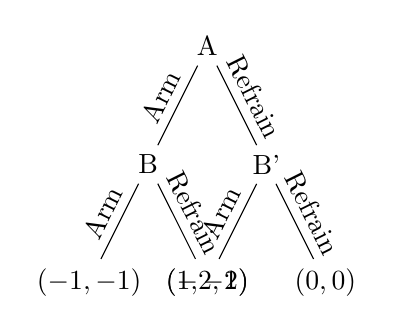
\begin{tikzpicture}[sloped]               
                \node {A}
                        child {                                
                                node {B}
                                        child {                
						node {$(-1,-1)$} 
						edge from parent
                                                        node[above] {Arm}
                                                }
                                        child {                 
						node {$(1,-2)$} 
						edge from parent
                                                        node[above] {Refrain}
                                                }
						edge from parent
                                                        node[above] {Arm}
                                }
                        child {                                
                                node {B'}
                                        child {                 
						node {$(-2,1)$} 
						edge from parent
                                                        node[above] {Arm}
                                                }
                                        child {                 
						node {$(0,0)$}
						edge from parent
                                                        node[above] {Refrain}
                                                }
						edge from parent
                                                        node[above] {Refrain}
                                };
        \end{tikzpicture}

	\begin{table}[h]
		\renewcommand{\arraystretch}{1,25}
	\begin{center}
	\begin{tabular}{crcccc}
		& & \multicolumn{4}{c}{B}\\
		& & (Arm, Arm') & (Arm, Refrain') & (Refrain, Arm') & (Refrain, Refrain')\\
		\cline{3-6}
		\multirow{2}{*}{A} & Arm & \multicolumn{1}{|c|}{$-1,-1$} & \multicolumn{1}{c|}{$-1,-1$} & \multicolumn{1}{c|}{$1,-2$} & \multicolumn{1}{c|}{$1,-2$}\\
		\cline{3-6}
		& Refrain & \multicolumn{1}{|c|}{$-2,1$} & \multicolumn{1}{c|}{$0,0$} & \multicolumn{1}{c|}{$-2,1$} & \multicolumn{1}{c|}{$0,0$}\\
		\cline{3-6}
	\end{tabular}
	\end{center}
	\end{table}

	\begin{itemize}
	\setlength\itemsep{0cm}
		\item In simultaneous games: \textit{Strategy} = \textit{Action}. This isn't the case in sequential games. \textit{Actions} are a simple move; \textit{Strategies} are plans based on the move of the first player
		\item A's strategies: Arm, Refrain
		\item B's strategies: (Arm, Arm'), (Arm, Refrain'). (Refrain, Arm'), (Refrain, Refrain')
		\item \textit{Information Set}: don’t know which two nodes you are at
		\item \textit{Subgame}: the mini-looking games which B is playing under A
	\end{itemize}

		\subsubsection{Choosing An Option}

	Normal:

	\begin{table}[h]
                \renewcommand{\arraystretch}{1,25}
        \begin{center}
        \begin{tabular}{crcc}     
                & & \multicolumn{2}{c}{B}\\
                & & (Export) & (No Export)\\
                \cline{3-4}
		\multirow{2}{*}{A} & FDI & \multicolumn{1}{|c|}{$25,-5$} & \multicolumn{1}{c|}{$40,\underline{10}$}\\
                \cline{3-4}
		& Export & \multicolumn{1}{|c|}{$\underline{30},\underline{30}$} & \multicolumn{1}{c|}{$\underline{60},10$}\\
                \cline{3-4}
        \end{tabular}
        \end{center}
        \end{table}

	Extensive:

	\tikzstyle{level 1}=[level distance=2cm, sibling distance=8cm]
        \tikzstyle{level 2}=[level distance=2cm, sibling distance=4cm]

        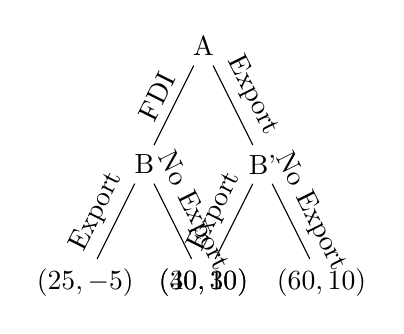
\begin{tikzpicture}[sloped]               
                \node {A}
                        child {                                
                                node {B}
                                        child {                
						node {$(25,-5)$} 
                                                edge from parent
                                                        node[above] {Export}
                                                }
                                        child {                 
                                                node {$(40,10)$} 
                                                edge from parent
                                                        node[above] {No Export}
                                                }
                                                edge from parent
                                                        node[above] {FDI}
                                }
                        child {                                
                                node {B'}
                                        child {                 
                                                node {$(30,30)$} 
                                                edge from parent
                                                        node[above] {Export}
                                                }
                                        child {                 
                                                node {$(60,10)$}
                                                edge from parent
                                                        node[above] {No Export}
                                                }
                                                edge from parent
                                                        node[above] {Export}
                                };
        \end{tikzpicture}

	\begin{itemize}
	\setlength\itemsep{0cm}
		\item In \textit{Normal Form}, (Export, Export) is the \textit{Dominant Strategy}, but there are more options:
		\begin{itemize}
			\item (Export, Export')
			\item (Export, No Export')
			\item (No Export, Export')
			\item (No Export, No Export')
		\end{itemize}
		\item If A plays FDI, will B ever export?
		\begin{itemize}
			\item (No Export, Export') allows \textit{Incredible Threats} to be made
		\end{itemize}
	\end{itemize}

		\subsubsection{Backwards Induction}

	\begin{itemize}
	\setlength\itemsep{0cm}
		\item A process used to avoid \textit{Incredible Threats}
		\item If A assumes B is rational, they expect B to play $(40,10)$ on FDI and $(30,30)$ on Export
		\item \textit{Credible Threats}:
		\begin{itemize}
			\item Only on FDI as they could lower their payoff to punish A
			\item $(25,-5)$
		\end{itemize}
	\end{itemize}

	\begin{enumerate}
	\itemsep\setlength{0cm}
		\item Start on that last stage of the game
		\item Break down into two of A's options
		\item Select these two \textit{Subgame Nash Equilibria} for B on each A arm
		\begin{itemize}
			\item (No Export, Export') are the best for B here
		\end{itemize}
		\item A now has a choice
		\begin{itemize}
			\item FDI would be followed by B's  No Export $(40,10)$ [$>(25,-5)$]
			\item Export would be followed by B's Export' $(30,30)$ [$<(60,10)$]
			\item A plays FDI
		\end{itemize}
		\item \textit{Nash Equilibrium} is made clear
		\begin{itemize}
			\item \{FDI,(Not Export, Export')\}
		\end{itemize}
	\end{enumerate}

		\subsubsection{Order Advantages}

	\begin{itemize}
	\setlength\itemsep{0cm}
		\item \textit{Commitment} in first mover vs. \textit{Flexibility} in follower
		\begin{itemize}
			\item Commitment has greater value in simultaneous games 
			\item Flexibility has greater value in sequential games
		\end{itemize}
		\item Recall that in simultaneous games there’s a first mover advantage
		\item \textit{First Mover Advantage} (Simultaneous):
		\begin{itemize}
			\item \begin{center}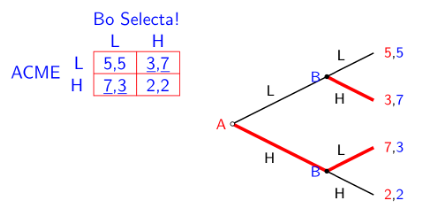
\includegraphics[width=6cm,height=3cm]{EC315-IMG/2.png}\end{center}
			\item B maximises on both moves and A maximises on its one move
			\item A lowers B’s payoff by choosing a more profitable option for them
		\end{itemize}
		\item \textit{Second Mover Advantage} (Sequential):
			\begin{itemize}                      
                        \item \begin{center}
\includegraphics[width=6.5cm,height=3cm]{EC315-IMG/3.png}\end{center}
                        \item M goes for overall highest payoff (6) by choosing move A
                        \item P has the option to choose one which greater benefits them and lowers M’s expected payoff
                \end{itemize}
	\end{itemize}

		\subsubsection{Manipulating Games}

	\begin{itemize}
	\setlength\itemsep{0cm}
		\item Take actions to manipulate a game? That is, guaranteeing the outcome
		\item \textit{Threats \& Promises}
		\begin{itemize}
			\item ``If you attack, I'll fight...''
			\item ``If you enter, I'll enter too; making it less profitable for you...''
			\item ``If you work hard, I'll work harder...''
			\item These lack credibility as they could be bluffs
		\end{itemize}
		\item \textit{Credibility}
		\begin{itemize}
			\item ``If you're late, I'll set off a bomb...'' (\textit{Incredible}; bluffing / not factual?)
			\item ``If you're late, the timed boomb will go off...'' (\textit{Credible}; more believable / factual)
			\item Changes first mover's thinking
		\end{itemize}
	\end{itemize}

		\subsubsection{Price Matching Guarantees}
	
	Standard \textit{Subgame Perfect Nash Equilibrium}:

	\begin{center}
		
\includegraphics[width=6cm,height=3cm]{EC315-IMG/4.png}
	\end{center}

	Offering a \textit{Price Match Guarantee}:

	\begin{center}
		
\includegraphics[width=4.5cm,height=6cm]{EC315-IMG/5.png}
	\end{center}

	\begin{itemize}
	\setlength\itemsep{0cm}
		\item Commitment to maintain high prices
		\item By committing to match low prices, A changes payoffs such that it’s not beneficial for B to undercut – as bigger payoff can’t be seen 
		\item Both firms end up paying high prices
		\item (Pricing) \textit{Prisoner’s Dilemma}
	\end{itemize}

	\newpage

	\subsection{Prisoner's Dilemma}

	\begin{itemize}
	\setlength\itemsep{0cm}
		\item \textit{Cooperate} or \textit{Defect}
		\item Mutual gain: \textit{Cooperate}
		\item Individual incentive: \textit{Defect}
		\item \textit{Pareto Efficienct Equilibrium}
		\item Recall: someone has a dominant strategy where there’s harm done to each other and they could be better off (Pareto Efficient). Self-interest doesn’t pay off. But, games can be repeated (e.g. price re-setting), e.g. lower price than opponent now (get more custom volume), makes opponent less-off (also poor for aggregate prices), firms may form a passive collusion where they both think opponents will set low so they both set high
		\item Both players have dominant strategy to defect but they could have a better result when the both cooperate. Hence, when choosing best interest, harm is done to the opponent when choosing to Defect for own interest, the opponent may choose to Cooperate so have a worse outcome
	\end{itemize}

	\begin{center}
		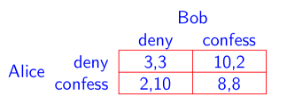
\includegraphics[width=5cm,height=2cm]{EC315-IMG/6.png}
	\end{center}

	Example:

	\begin{enumerate}
	\setlength\itemsep{0cm}
		\item (8,8) is Pareto Inefficient equilibrium as it is reached by both aiming for low by confessing. Could be made better off by both acting for mutual gain (3,3)
		\item Pricing – non-brand loyal market, flow freely between

		\item Team Work – (work vs shirk) shirk leads to more payoff as still full marks but no work done but if the other does all the work, they will get full marks but payoff will reduce due to workload
		\item Clean vs Dope – (risk based) best self-interest response is to dope as highest possible payoff but the equilibrium they both do it is less than the payoff if they both don’t
		\item Market Share – studying marketing is a waste of time. Market is a pie, we compete over our share. Ads try to [1] inform and [2] predatory (winning market share). Start: 50/50, engage in ads to win market share. I spend money, I get some in return but you won’t gain much more market share. The opponents do this to keep up. Each keep catching back up to 50\% each but both are still wasting millions on marketing. Market share isn’t changing proportionately but you’re still spending money
	\end{enumerate}

	\begin{center}
		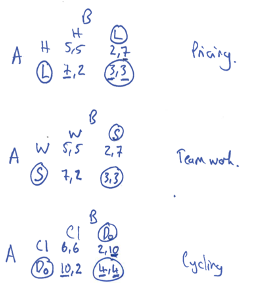
\includegraphics[width=3.5cm,height=4.5cm]{EC315-IMG/7.png}
	\end{center}

		\subsubsection{Externalities}

	\begin{itemize}
        \setlength\itemsep{0cm}
		\item \textit{Negative Externalities}: (own interest – doing too much) Cooperation reduces amount of work you do for the better (e.g. not over-fishing)
		\begin{itemize}
			\item Don’t see costs from defecting – too much harmful activity is done
		\end{itemize}
		\item \textit{Positive Externalities}: (own interest – doing too little) Cooperation says you should do more work (e.g. not doing no work in a project)
		\begin{itemize}
                        \item Don’t see costs benefits form cooperating – too little of a good activity is done
                \end{itemize}
		\item Example: Marginal Benefit vs. Marginal Cost – (1) extracting fish from the ocean makes it harder in the future (e.g. do less fishing to allow repopulation). (2) But you want more to sell now. (3) Self-interest makes it harder for others
	\end{itemize}

		\subsubsection{Rationalise Cooperation Resolutions}

	\begin{itemize}
        \setlength\itemsep{0cm}
		\item Resolutions to \textit{Prisoner's Dilemma}
		\item Meet-up (verbal agreement): let’s set high prices (incentive of deception however – you want him to set high prices and you want to set low)
		\item \textit{Threaten}: punishment of opponent doesn’t set high prices (lacking credibility as you ``will do it'' rather than it ``will be done (automatically etc.)'' – can fix credibility by using Mafia as they have more incentive to harm him)
		\item \textit{Reward}: offer a reward that overcomes the incentive to defect (still lacks credibility as it involves giving money – lowers your payoff. May not even believe you)
	\end{itemize}

		\subsubsection{Behavioural Resolution}
	
	\begin{itemize}
        \setlength\itemsep{0cm}
		\item \textit{External Norms of Behaviour}: Think back to litter e.g.: many people won’t actually litter even though it’s the most beneficial for you. It conflicts with the social norm
		\item \textit{Internal Norms of Behaviour}: Doing nice things for people who are nice to you (gain utility). Being bad to people but they are good to you (loss of utility). - you defect but if you care enough, you’ll maybe rationalise cooperation and change mind
	\end{itemize}

		\subsubsection{Price Matching Guarantee Resolution}

	\begin{itemize}                                         
        \setlength\itemsep{0cm}
		\item You may be undercut for opponent to gain market share from you at lower prices
		\item If you’re offered. PMG, you will simply match prices and keep customers ``he’s selling at that price, can you just sell me at that too''
		\item Opponent now doesn’t gain, just sells at lower price as no market gain
		\item Equilibrium of both pricing high – out of Prisoner’s Dilemma
	\end{itemize}

	\begin{center}
		
\includegraphics[width=4cm,height=4cm]{EC315-IMG/10.png}
	\end{center}

		\subsubsection{Dynamic Punishment Resolution}

	\begin{itemize}                                         
        \setlength\itemsep{0cm}
		\item When defecting, a player may believe they will be ‘punished’ in the future
		\item Can we achieve cooperation through fear of punishment?
		\begin{itemize}
			\item Credible: backed with fact
			\item Incredible: maybe won’t happen 
		\end{itemize}
		\item \textit{Finite Period} ($T$ Periods): defect in last period as no more time for retaliation
		\begin{itemize}
			\item Final period: mutual dominant strategy to defect as no future punishment 
			\item So: best to defect this period as well as you both will next
		\end{itemize}
		\item \textit{Infinite Period}: the game will continue [probability $p=1$] so retaliation 
		\begin{itemize}
			\item Always an opportunity to punish as there’s always another period
		\end{itemize}
		\item \textit{Impatient}: future worth less than present so defect (not caring for punishment)
		\item \textit{Patient}: care more for future gain by waiting and cooperating
	\end{itemize}
		
		\paragraph{Discounting}

	\begin{itemize}
	\setlength\itemsep{0cm}
		\item \pounds1 from \pounds1 today to \pounds1($1+r$) tomorrow; \pounds1 from \pounds1 tomorrow to \pounds$\frac{1}{(1+r)}$ today
		\item PV: $\frac{1}{(1+r)}$, $\frac{1}{(1+r)^2}$, ..., $\frac{1}{(1+r)^N}$; for discount rate $r$ and discount factor $\delta=\frac{1}{(1+r)^t}$
		\item Hence, \pounds$X$ in period $t$ is worth \pounds$X\frac{1}{(1+r)^t}$ today
		\item Hence, \pounds$X$ in period $t$ is worth \pounds$X\delta^t$ today
		\item $\delta$ close to 1: patient; $\delta$ close to 0: impatient
		\item CFs: $X_0,X_1,...,X_N$; PVs: $X_0+\delta X_1+\delta^2X_2+,...,+\delta^NX_N$
		\item Infinite: $1+\delta+\delta^2+\delta^3=\frac{1}{(1-\delta)}$
	\end{itemize}

	Example:

	\begin{center}
		
\includegraphics[width=6cm,height=2cm]{EC315-IMG/11.png}
	\end{center}

	\begin{center}
	\begin{tabular}{l|l}
		Payoff of 7 in perpetuity & Payoff of 10 today and 2 in perpetuity\\
		$7+7\delta+7\delta^2+...=7\frac{1}{1-\delta}$ & $10+2\delta+2\delta^2+...=10+2\delta\frac{1}{(1-\delta)}$
	\end{tabular}
	\end{center}

	\newpage

		\paragraph{Trigger Strategies: Grim Trigger}

	\begin{itemize}                
        \setlength\itemsep{0cm}
		\item Start by cooperating
		\item If opponent cooperated, cooperate
		\item If opponent defected, defected in perpetuity
	\end{itemize}

	\begin{enumerate}                                      
        \setlength\itemsep{0cm}
		\item \textit{Cooperate}:
		\begin{itemize}
			\item Opponent gets 600 forever $\rightarrow$ $600+600\delta+600\delta^2+...=\frac{600}{(1-\delta)}$
		\end{itemize}
		\item \textit{Defect}:
		\begin{itemize}                            
			\item Get 1000 now but 400 after $\rightarrow$ $1000+400\delta+400\delta^2+...=1000+\frac{400\delta}{(1-\delta)}$
                \end{itemize}
		\item Answer:
		\begin{itemize}                            
			\item $\frac{600}{(1-\delta)}\ge1000+\frac{400\delta}{(1-\delta)}\Leftrightarrow\delta\ge\frac{2}{3}(\Leftrightarrow\le\frac{1}{2})$ = 50\%
			\item \fbox{Hence, \textit{Grim Trigger} at $\delta>\frac{2}{3}$ so cooperate}
                \end{itemize}
	\end{enumerate}

		\paragraph{Trigger Strategies: Tit-for-Tat}

	\begin{itemize}
	\setlength\itemsep{0cm}                             
                \item Start by cooperating
		\item Play as the opponent played in the last round
		\item Cooperation followed by cooperation
		\item Defection frollowed by defection 
	\end{itemize}

	\begin{enumerate}                              
        \setlength\itemsep{0cm}                                   
                \item \textit{Defect} in perpetuity:                         
                \begin{itemize}                        
			\item Same as Grim Trigger: $\delta\ge\frac{2}{3}$
                \end{itemize}   
                \item \textit{Defect} once:
                \begin{itemize}       
			\item Get 400 now but loses 430 after $\rightarrow$ $400\le430\delta\Rightarrow\delta\ge\frac{40}{43}(\Rightarrow\le0.075)$ = 7.5\%
                \end{itemize}                              
                \item Answer:
                \begin{itemize}
                        \item \fbox{Hence, \textit{TFT} at $\delta>\frac{40}{43}$ so cooperate}
		\end{itemize}
        \end{enumerate}

	\fbox{If \textit{Grim} works: cooperation possible; If \textit{TFT} works: cooperation easy}

	\newpage

	\subsection{Games With Continuous Strategies}

	\begin{itemize}
	\setlength\itemsep{0cm}
		\item This is applying maths to what we already know
		\item Nash equilibriums and sub-game perfect nash equilibriums remain the same
		\item This is applying the following more generally  
		\item Matrix strategy: can choose any option for the expected opponent’s options
		\begin{itemize}
			\item Simultaneous: best responses and mutually consistent best responses
			\item Sequential: backward induction 
		\end{itemize}
		\item Take a long time to analyse a continuous strategy using discrete sets (matrix)
	\end{itemize}

		\subsubsection{Quantity Competition}

	\begin{itemize}
	\setlength\itemsep{0cm}
		\item In a \textit{Competitve Market}
		\item Firm $i$ supplies $q_i$ (where $\sum_{i=1}^Nq\ \forall i\{1,...,N\}$)
		\item \textit{Inverse Demand Function}: $p(Q)=a-bQ$
		\item Payoff is \textit{Profit} ($\pi_i$): $q_ip(Q)-C_i(q_i)$
		\item Hence: $\pi_i(q_{i=1},q_{i=2},...,q_N)=q_ip(Q)-C_i(q_i)$
		\item There is an \textit{Oligopoly} if several firms compete
		\item This method is shown in 1 to $N$ matrices for A to respond to B:
		\item 
			\begin{center}
			\begin{tabular}{ccc}
				
\includegraphics[width=5cm,height=2cm]{EC315-IMG/12.png} & $\longrightarrow$ & 
\includegraphics[width=5cm,height=2cm]{EC315-IMG/13.png}\\
			\end{tabular}
			\end{center}
		\item Hence, we find a \textit{Payoff Function} which is maximised at a point; ``find the level of $q_1$ maximising firm A's payoff for given $q_2$''
	\end{itemize}

		\subsubsection{Continuous Strategies}

	\begin{itemize}
        \setlength\itemsep{0cm}
		\item Too hard to account for all the options (in this case quantities to produce)
		\item Recall basic math: \textit{Function}: the level; \textit{Derivative}: the slope of the function; \textit{Parital Derivative}: fix a variable
	\end{itemize}

		\paragraph{Rules of Differentiation}

	\begin{itemize}
	\setlength\itemsep{0cm}
		\item Woring towards \textit{Payoff Function}
		\item Just like in the matrixes, fix the opponents option each time to find your best
		\item Hence, $y=f(x_1,x_2)$
		\item Fix $x_2$ (the adjacent firm's strategy) to observe how $x_1$ varies with $y$
		\item Therefore, partial derivative $\frac{\partial y}{\partial x_1}$ for fixed $x_2$
		\item Thus, best response at $\{\frac{\partial y}{\partial x_1}|_{x_2}=0\}$ (peak of function)
		\item Note that, if you take the derivative on the incline of the function, you can be made better off by doing more. Take the derivative on the decline, better off by doing less
		\item 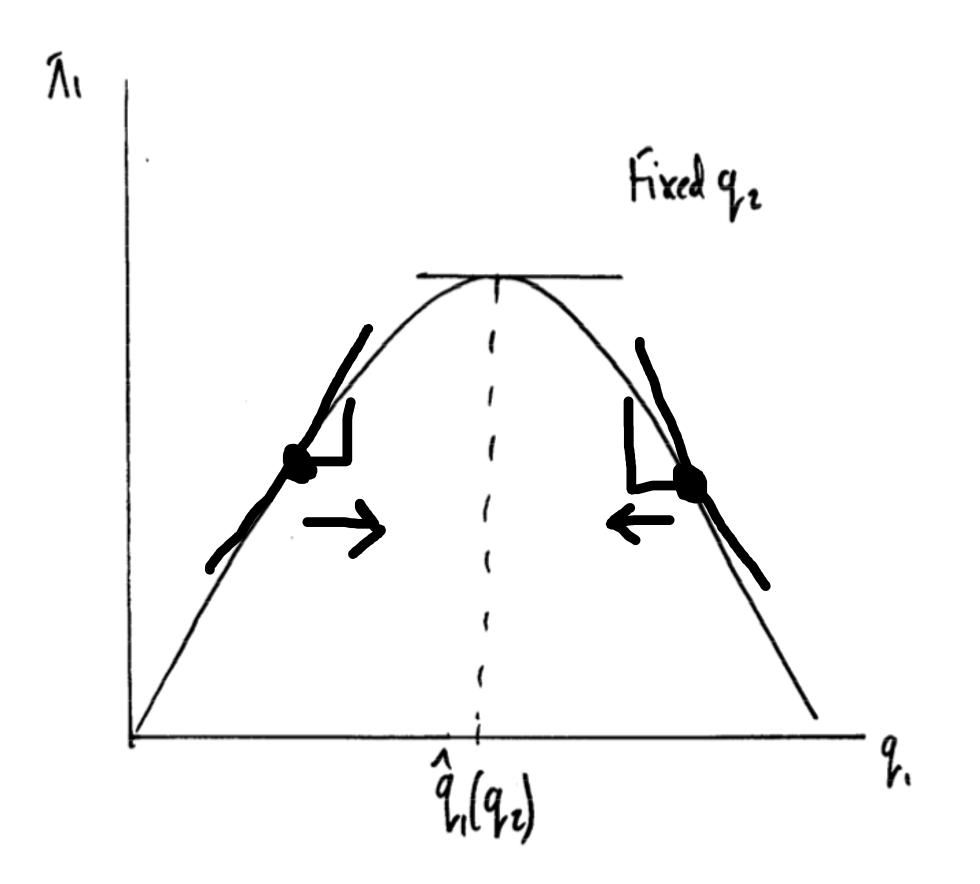
\includegraphics[width=3.5cm,height=3cm]{EC315-IMG/14.png}
	\end{itemize}

	\begin{itemize}                              
        \setlength\itemsep{0cm}
		\item Recall the function $f(x)$:
		\begin{itemize}
			\item $f'(x)$ positive at incline
			\item $f'(x)$ negative at decline
			\item $f'(x)=0$ at stationery point (max/min)
			\item 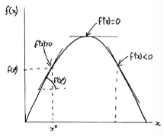
\includegraphics[width=3.5cm,height=3cm]{EC315-IMG/15.png}
		\end{itemize}
		\item Recall if $f(x)=x^n$ then $f'(x)=nx^n-1$
		\begin{itemize}
			\item Constant: $ch(x)\longrightarrow ch'(x)$
			\item Sum: $g(x)\pm h(x)\longrightarrow g'(x)\pm h'(x)$
			\item Product: $g(x)h(x)\longrightarrow g(x)h'(x)+g'(x)h(x)$
			\item Chain: $g(h(x))\longrightarrow g'(h(x))h'(x)$
			\item Quotient: $\frac{g(x)}{h(x)}\longrightarrow\frac{g'(x)h(x)-g(x)h'(x)}{{h(x)}^2}$
			\item Log: $\ln x\longrightarrow\frac{1}{x}$
		\end{itemize}
		\item In practice:
		\begin{itemize}
			\item Power: $\sqrt{x}=x^{\frac{1}{2}}\longrightarrow\frac{1}{2}x^{-\frac{1}{2}}=\frac{1}{2\sqrt{x}}$
			\item Constant: $3x^2\longrightarrow3\times2x$
			\item Sum: $x^2+x^3\longrightarrow 2x+3x^2$
			\item Product: $x^2(2x+3)^9\longrightarrow x^2\times9(2x+3)^8\times2+(2x+3)^9\times2x$
			\item Chain: $x^2(2x+3)^9\longrightarrow9(2x+3)^8\times2$
			\item Quotient: $\frac{x}{(1+x)}\longrightarrow\frac{(1+x)\times(1-x)\times1}{(1+x)^2}$
		\end{itemize}
	\end{itemize}

		\subsubsection{Cournot Derivation of Payoff \& Reaction (Simultaneous)}
	
		\paragraph{Step 1}

	\textit{Fix firm 2's action and find firm 1's best response to it.}

	\begin{itemize}
	\setlength\itemsep{0cm}
		\item Find \textit{Payoff Function}
		\item Partially derive and $=0$ for \textit{Best Response} with fixed $q_2$
		\item Find best $q_1$ for \textit{Reaction Function}, sub for $q_1^*$
	\end{itemize}
		
		\paragraph{Step 2}

	\textit{Fix firm 1's action and find firm 1's best response to it.}

	\begin{itemize}
        \setlength\itemsep{0cm}
                \item Find \textit{Payoff Function}
		\item Partially derive and $=0$ for \textit{Best Response} with fixed $q_1$
		\item Find best $q_2$ for \textit{Reaction Function}, sub for $q_2^*$
	\end{itemize}

		\paragraph{Step 3}

	\textit{Find meeting point of Nash Equilibrium where Reaction Functions meet; substitute to find optimal $\pi$ for each firm.}

		\paragraph{Definitions}

	\begin{itemize}                                                    
        \setlength\itemsep{0cm}                                            
                \item Players: 2 firms $i=1,2$
		\item Strategies: each firm chooses quantity of $q_i$, for $Q=q_1+q_2$
		\item Payoff: given supply choices \textit{Marginal Cost} of $c$, \textit{Price} of $P(q_1+q_2)$, \textit{Payoff} (profit) of $\pi_i(q_1,q_2)=q_1p(q_1+q_2)-cq_i$
	\end{itemize}

		\paragraph{Working Example}

	Firm 1's \textit{Payoff Function}: $\pi_1=q_1(a-b(q_1+q_2))-cq_1$\\
	$\pi_1=q_1(a-bq_1-bq_2)-cq_1$\\
	$\pi_i=aq_1-bq_1^2-bq_1q_2-cq_1$\\

	Fix $q_2$: $\frac{\partial\pi_1}{\partial q_1}=a-2bq_1-bq_2-c$\\
	$[a-2bq_1-bq_2-c=0]$\\
	$[2bq_1=a-c-bq_2]$\\

	Firm 1's \textit{Reaction Function}: $[q_1=\frac{a-c-bq_2}{2b}]...[q_1=\frac{a-c}{2b}-\frac{1}{2}q_2]$\\
	Recall: $q_1$ is not $(-)$ as $q_2\le\frac{a-c}{b}$\\

	Note that \textit{Reaction Function}: $q_1^*=\hat{q}_1(q_2)=\begin{Bmatrix}\frac{a-c}{2b}-\frac{1}{2}q_2\mathrm{if}q_2\le\frac{a-c}{b}\\0\mathrm{if}q_2>\frac{a-c}{b}\end{Bmatrix}$\\

	Hence, \textit{Reaction Function}: output quantity should decline as the opponent's increases; when it reaches 0, leave market; obviously no negative

	\begin{center}
		
\includegraphics[width=3cm,height=3cm]{EC315-IMG/16.png}
	\end{center}

	Firm 2's \textit{Payoff Function}: $\pi_2=q_2(a-b(q_1+q_2))-cq_2$\\
	Fix $q_1$: $\frac{\partial\pi_2}{\partial q_2}=a-2bq_2-bq_1-c$\\
	Firm 2's \textit{Reaction Function}: $[q_2=\frac{a-c-bq_1}{2b}]...[q_2=\frac{a-c}{2b}-\frac{1}{2}q_1]$\\

	Note that \textit{Reaction Function}: $q_2^*=\hat{q}_2(q_1)=\begin{Bmatrix}\frac{a-c}{2b}-\frac{1}{2}q_1\mathrm{if}q_2\le\frac{a-c}{b}\\0\mathrm{if}q_1>\frac{a-c}{b}\end{Bmatrix}$
	
	\begin{center}
                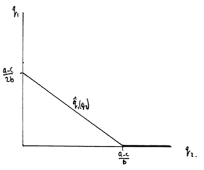
\includegraphics[width=3cm,height=3cm]{EC315-IMG/17.png}
        \end{center}

	\textit{Nash Equilibrium} (``The Courot Equilibrium''): flip firm 2's \textit{Reaction Function} and overlay\\
	Seek $q_1^*,q_2^*$ from $q_1^*=\hat{q}_1(q_2^*)$ and $q_2^*=\hat{q}_2(q_1^*)$\\
	``For firm 1's $q$ which maximises its $\pi$ given firm 2's $q$''\\
	``For firm 2's $q$ which maximises its $\pi$ given firm 1's $q$''

	\begin{center}
                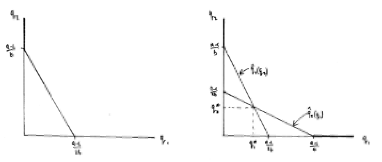
\includegraphics[width=7cm,height=3cm]{EC315-IMG/18.png}
        \end{center}

	\textit{Substitution} is as follows:\\
	From $q_1=\frac{a-c}{2b}-\frac{1}{2}q_2$\\
	$q_1=\frac{a-c}{2b}-\frac{1}{2}(\frac{a-c}{2b}-\frac{1}{2}q_1)$\\
	$q_1=\frac{a-c}{2b}-\frac{a-c}{4b}+\frac{1}{4}q_1$\\
	$q_1=\frac{4b\left(a-c\right)-2b(a-c)}{8b^2}+\frac{1}{4}q_1$\\
	$q_1=\frac{2b\left(a-c\right)}{8b^2}+\frac{1}{4}q_1$\\
	$q_1=\frac{a-c}{4b}+\frac{1}{4}q_1$\\
	${\frac{3}{4}q}_1=\frac{a-c}{4b}$\\
	$q_1=\frac{4}{3}\frac{a-c}{4b}$\\
	$q_1=\frac{4(a-c)}{12b}$\\
	$q_1^*=\frac{a-c}{3b}$
	Sub for firm 2's $\pi$

	\textit{Cournot Equilibrium} is as follows:
	Hence: $Q^*=q_1^*+q_2^*$\\
	So: $p^*=a-bQ^*$\\
	Thus: $\pi^*=(p^*-c)Q^*$\\

	\fbox{$q_1^*=q_2^*=\frac{a-c}{3b}$; $Q^*=\frac{2(a-c)}{3b}$; $p^*=\frac{a+2c}{3}$; $\pi_i^*=\frac{(a-c)^2}{9b}$}\\

	Verify that:\\
	Industry output between monopoly and PC: $Q^M<Q^\ast+Q^C$\\
	Price between monopoly and PC: $p^M=p^\ast+p^C$\\
	Industry profit between monopoly and PC: $\pi^M>{\pi_1}^\ast+{\pi_2}^\ast>0$

		\subsubsection{Stakleberg Leader \& Follower (Sequential)}

	\begin{itemize}
	\setlength\itemsep{0cm}
		\item The leader implements the first player’s reaction function intro their payoff function 
		\item First mover advantage as leader gets higher payoff
		\item Recall from sequential games: backward induction
		\item \textit{Linear Demand}: $P(Q)=a-bQ$
		\item \textit{Constant Marginal Costs}: $C_i(q_i)=cq_i$
		\item \textit{Profits}: $\pi_i(q_i,q_j)=q_i\left(a-b(q_i+q_j)\right)-cq_i$
		\item Firm 1 moves, firm 2 observes and moves
		\item Firm 1 is the leader, firm 2 is the follower
		\item Recall:
		\item 
\includegraphics[width=3.5cm,height=3cm]{EC315-IMG/19.png}
	\end{itemize}

		\paragraph{Backward Induction: Step 1 (Stage 2)}

	\begin{itemize}
	\setlength\itemsep{0cm}
		\item Firm 2 maximises profits given $q_1$
		\item Firm 2 uses Best Response to whatever firm 1 produces
	\end{itemize}

	\begin{enumerate}
        \setlength\itemsep{0cm}
		\item Recall: $\pi_2=q_2(a-b(q_1+q_2))-cq_2$ (\textit{Payoff Function})
		\item Optimise and $=0$: $\frac{\partial_{\pi2}}{\partial_{q2}}=a-2{bq}_2-bq_1-c=0$
		\item React: ${q_2}^\ast={\hat{q}}_2\left(q_2\right)=\frac{a-c}{2b}-\frac{1}{2}q_1$ (\textit{Reaction Function})
	\end{enumerate}

	\newpage

		\paragraph{Backward Induction: Step 2 (Stage 1)}

	\begin{itemize}
	\setlength\itemsep{0cm}
		\item Firm 1 anticipates reaction of firm 2 to any decision made
		\item Firm 1 maximises profits given response of firm 2
		\item Firm 1 chooses point on firm 2’s reaction function which maximises profits
	\end{itemize}
	
	\begin{enumerate}                                       
        \setlength\itemsep{0cm}
		\item Recall: $\pi_1(q_1{,q}_2)=q_1(a-b(q_1+q_2))-cq_1$ (\textit{Payoff Function})
		\item It Knows: if they choose $q_1$ firm 2 will respond with ${q_2}^\ast={\hat{q}}_2({q_1}^\ast)$
		\item Firm 1 (leader): $\pi_1(q_1{,\hat{q}}_2(q_1))=q_1(a-b(q_1+{\hat{q}}_2(q_1)))-cq_1$
		\begin{itemize}
			\item Therefore: $\pi_1\left(q_1{,\hat{q}}_2\left(q_1\right)\right)=\frac{a-c}{2}q_1-\frac{b}{2}q_1^2$
		\end{itemize}
		\item So firm 1 maximises: $\frac{\delta_{\pi1(q1,q2)}}{\delta_{q1}}=\frac{a-c}{2}-{bq}_1=0$
		\begin{itemize}
			\item Therefore: $q_1^L=\frac{a-c}{2b}$ (\textit{Reaction Function})
		\end{itemize}
		\item So firm 2 (follower): $q_2^F=\frac{a-c}{2b}-\frac{1}{2}q_1^L$
		\begin{itemize}
			\item $q_2^F=\frac{a-c}{4b}$
		\end{itemize}
	\end{enumerate}

		\paragraph{Stakleberg Equilibrium}

	\textit{``Rather than an equilibrium, there is an advantage''}\\

	\fbox{$Q^S=\frac{3(a-c)}{4b}$; $\pi_1^L=\frac{{(a-c)}^2}{8b}$; $\pi_2^F=\frac{{(a-c)}^2}{16b}$}

		\paragraph{Stakleberg vs. Cournot}

	Cournot: $q_1^\ast=q_1^\ast=\frac{a-c}{3b}$; $Q^\ast=\frac{2(a-c)}{3b}$; $p^\ast=\frac{a+2c}{3}$; $\pi_1^\ast=\pi_2^\ast=\frac{{(a-c)}^2}{9b}$\\
	
	Stakleberg:
	\begin{tabular}{ll}
		$q_1^L=\frac{a-c}{2b}>q_1^\ast$; & $q_2^F=\frac{a-c}{4b}<q_2^\ast$;\\
		$Q^S=\frac{3(a-c)}{4b}>Q^\ast$; & $p^S=\frac{a+3c}{4}<p^\ast$;\\
		$\pi_1^L=\frac{(a-c)^2}{8b}>\pi_1^\ast$; & $\pi_2^F=\frac{(a-c)^2}{16b}<\pi_2^\ast$
	\end{tabular}\\
	
	Hence, first mover (firm 1) advantage
	
	\newpage

	\subsection{Applications of Prisoner's Dilemma}

	\begin{itemize}
	\setlength\itemsep{0cm}
		\item An example of a continuous game
		\item Rather than using \textit{Reaction Functions}, find \textit{Isoprofit Curves}
		\item This is like indifference curves for firms
		\item Call firms $i,j$; strategies $x_i,x_j$; payoffs $\pi(x_i,x_j)$
	\end{itemize}

		\subsubsection{Typical Reaction Function}

	$${\hat{q}}_i\left(q_j\right)=\frac{a-c}{2b}-\frac{1}{2}q_j$$
	
	From \textit{Isoprofit} contours\\
	Equilibrium at intersection: $q_i^\ast=q_j^\ast=\frac{a-c}{3b}$

		\subsubsection{Maximising Joint Profit}

	$$J\left(q_i,q_j\right)=\left(q_i+q_j\right)\left(a-b(q_i+q_j)\right)-{cq}_i-{cq}_j$$

	$\frac{\partial J}{\partial q_i}=a-2b\left(q_i+q_j\right)-c=0\rightarrow{\widetilde{q}}_i\left(q_j\right)=\frac{a-c}{2b}-q_i$\\
	$\frac{\partial J}{\partial q_j}=a-2b\left(q_i+q_j\right)-c=0\rightarrow{\widetilde{q}}_j\left(q_i\right)=\frac{a-c}{2b}-q_j$\\

	Hence, assuming $q_i=q_j=\widetilde{q}$\\
	$\widetilde{q}=\frac{a-c}{4b}$\\
	Makes sense as: $2\left(\frac{a-c}{4b}\right)=\frac{a-c}{2b}$ (Monopoly Output)

		\subsubsection{Will Firms Agree?}

	\begin{itemize}
	\setlength\itemsep{0cm}
		\item Will firms agree to produce at half the monopoly output?
		\item \textbf{No}; if firms expect you to produce more than $\widetilde{q}$;
		\item Best possible: ${\hat{q}}_i(\widetilde{q})$ $\rightarrow$ must expand output in excess of \textit{Cournot Output}
		\item Defecting firm: \textit{Bonanza Payoff}
		\item Cooperating firm: \textit{Sucker Payoff}
		\item Hence, \textit{Prisoner's Dilemma}
		\item $\pi^B>{\frac{1}{2}\pi}^M>\pi^\ast>\pi^S$
		\item 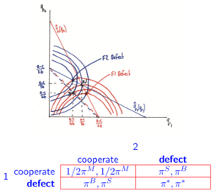
\includegraphics[width=4cm,height=4cm]{EC315-IMG/20.png}
	\end{itemize}

		\subsubsection{Externalities}

		\paragraph{Negative}

	You do more, you lower my payoff (\textit{Cournot Game})\\
	$\frac{\partial \pi_i}{\partial x_j}<0$ (slope of \textit{Payoff Function})

		\paragraph{Positive}

	You do more, you lower my payoff\\
	$\frac{\partial \pi_i}{\partial x_j}>0$ (slope of \textit{Payoff Function})

		\subsubsection{Strategic Nature}

		\paragraph{Strategic Substitutes}

	Opponent does more of their action: you optimally do less (\textit{Reaction Function} downward)\\
	$\left(\frac{\partial\frac{\partial \pi_i}{\partial x_i}}{\partial x_j}\right)<0$ ``with a higher $x_j$, the optimum is with a lower $x_i$''

		\paragraph{Strategic Compliments}
	
	Opponent does more of their action: you optimally do more (\textit{Reaction Function} upward)\\
	$\left(\frac{\partial\frac{\partial \pi_i}{\partial x_i}}{\partial x_j}\right)>0$ ``with a higher $x_j$ the optimum is with a higher $x_i$''

		\subsubsection{Nash Equilibrium in Games}

	\begin{itemize}
	\setlength\itemsep{0cm}
		\item When non-cooperative, players optimise self-interest
		\item Marginal Payoff $=0$: $\frac{\partial \pi_i}{\partial x_i}=0$; $\frac{\partial \pi_j}{\partial x_j}=0$
		\item Nash equilibrium at: ${\hat{x}}_i\left(x_j\right)$ and ${\hat{x}}_j(x_i)$
		\item Thus, nash equilibrium actions: $x_i^\ast,x_j^\ast$
	\end{itemize}

		\subsubsection{Social Planner}

	\begin{itemize}
	\setlength\itemsep{0cm}
		\item What happens when they `internalise' the externality?
		\item \textit{Social Planner} maximises joint payoff
	\end{itemize}

	$$J=\pi_i\left(x_i,x_j\right)+\pi_j\left(x_i,x_i\right)$$

	Chooses $x_i,x_j$ to maximise\\
	$\frac{\partial J}{\partial x_i}=\frac{\partial \pi_i}{\partial x_i}+\frac{\partial \pi_j}{\partial x_j}=0\rightarrow{\widetilde{x}}_i(x_j)$\\
	$\frac{\partial J}{\partial x_i}=\frac{\partial \pi_i}{\partial x_i}+\frac{\partial \pi_j}{\partial x_j}=0\rightarrow{\widetilde{x}}_i\left(x_j\right)$ $\rightarrow$ these are both \textit{Social Optimums}

		\subsubsection{Nash Equilibrium vs. Optimum}

		\paragraph{w/ Positive Externalities}

	$\frac{\partial \pi_j}{\partial x_i}>0$\\
	So for \textit{Social Planner} ($\frac{\partial \pi_i}{\partial x_i}$ must be $<$ NE)\\
	So ${\widetilde{x}}_i\left(x_j\right)>{\hat{x}}_i\left(x_j\right)$

		\paragraph{w/ Negative Externalities}
	
	$\frac{\partial \pi_j}{\partial x_i}<0$\\           
        So for \textit{Social Planner} ($\frac{\partial \pi_i}{\partial x_i}$ must be $>$ NE)\\
        So ${\widetilde{x}}_i\left(x_j\right)<{\hat{x}}_i\left(x_j\right)$

	\begin{center}
		
\includegraphics[width=5cm,height=4.5cm]{EC315-IMG/21.png}
	\end{center}

\newpage

...

\newpage

\section{Cross-Section Econometrics}

	\subsection{Descriptive Statistics}

	\begin{center}
                \scriptsize
        \begin{longtable}{p{3cm}p{9cm}}
                \hline
                \hline
	       	\multicolumn{2}{c}{\textbf{Variable Types}}\\
                \hline
                \hline
                \multicolumn{2}{c}{\textbf{Numerical}}\\
                \hline
                Continuous & Infinite possible values.\newline Real line or interval.\newline E.g. page number on your Beamer slide show or; hh:MM:SS:ss -- dd/mm.yyyy.\\
                Discrete & Restricted possible values.\newline Bound to lower and upper limit.\newline E.g. number of lexer errors in {\TeX} log when you try to use HTML shortcuts as opposed to basic Unicode shortcuts.\\
                \hline
                \multicolumn{2}{c}{\textbf{Categorical}}\\
                \hline
                Ordinal & Ordered/sequenced and has meaning.\newline E.g. gender, race, eye colour etc.; any type of group residence.\\
                Regular & Ordered/sequenced and has no meaning.\newline E.g. surname, forename.\\
                \hline
                \multicolumn{2}{c}{\textbf{Relationships}}\\
                \hline
                Correlation & How variables move together (direction).\newline Correlation $\neq$ Causation\\
                Association & Intuitively connected but, perhaps, not correlated.\\
                Dependence & Does correlatively rely on the movement of another variable.\\
                Independence & Does not correlatively rely on the movement of another variable.\\
                \hline
                \hline
                \multicolumn{2}{c}{\textbf{Data Collection}}\\
                \hline
                \hline
                Sample & Portion of population selected for analysis.\newline Used to make assumptions and inference upon entire populations.\\
                Population & Entirety of the group from which a sample is extracted.\\
                \hline
                \multicolumn{2}{c}{\textbf{Sampling Bias}}\\
                \hline
		Non-Responsive & Only a small portion of a the proposed sample responded.\\
                Voluntary Response & Irrational bias in opinions of people within sample.\\
                Convenience & More accessibility leads to easier response. May lead to skewed results.\newline E.g. a farming survey’s results in Central Asia may be skewed towards commercial farming because of India (easier to survey), although subsistence farming is significantly more present in remote (harder to survey) areas such as Nepal; of which there is a larger quantity.\\
                Observations & Conductor observes information and translates it to data (observations) from existing scenario.\\
                Experiment & Conductor observes data from results of self-manufactured scenario.\\
                \hline
                \hline
                \multicolumn{2}{c}{\textbf{Examining Data}}\\
                \hline
                \hline
                Scatter Plot & Plots scattered across a 2D \textit{x}-axis/\textit{y}-axis\newline Allows for identification of relationship between \textit{x} (explanatory axis) and \textit{y} (response axis).\newline E.g. linear (positive/negative), polynomial (varying by degree \{quadratic, cubic, quartic, quintic, ...\}) etc.\\
                Bar Graph & Basic comparison of values (\textit{y}-axis) of categories (\textit{x}-axis).\\
                Population Pyramids & Comparison of intervals (\textit{y}-axis) across two categorical groups (\textit{x}-axis 1, \textit{x}-axis 2). Often used in human population.\\
                Box Plot & Highlights minimum, first quartile, median, third quartile and maximum.\\
                \hline
                \multicolumn{2}{c}{\textbf{Distribution Moments}}\\
                \hline
                Mean & $\mu=\frac{\Sigma x}{N}$ = Population Mean; $\bar{x}=\frac{\Sigma x}{n}$ = Sample Mean\newline Common `average’ value.\newline Supplies line of best fit in linear equations.\newline Influenced by outliers so can be skewed.\\
                Median & Central value in dataset.\newline Neglects outliers, to a degree (hence, used for salary etc.)\newline Finds quartile ranges: 0 - Q1 - Q2 - Q3 - N (IQR)\\
                Standard Deviation & $\sigma$ = Standard Deviation\newline How much data deviates from the mean.\newline Same units as the data.\\
                Variance & $\sigma^2$ = Variance\newline Fairly weighted measure of variation from the mean.\newline Discards negatives, weights higher deviations more.\\
                Covariance & $\mathrm{cov_{\textit{x,y}}=\sigma_\textit{x}\sigma_\textit{y}\rho_{\textit{x,y}}}$ = Covariance\newline Variation of members of the dataset, relative to others.\\
                Correlation & $\mathrm{\rho_{\textit{x,y}}=\frac{cov_{\textit{x,y}}}{\sigma_\textit{x}\sigma_{\textit{y}}}}$ = Correlation\newline If $\rho$ = 1: Perfect Positive Correlation (Together)\newline If $\rho$ = -1: Perfect Negative Correlation (Apart)\newline If $\rho$ = 0: No Correlation\newline Correlation Matrices map all possible movements together.\\
		Skewness & Degree of asymmetry around the mean.\newline \textbf{Symmetric: }assume mean in centred.\newline \{mean $\approx$ median\}; \{skewness $\approx$ 0\}\newline \textbf{Left Skewness: }tail to left \{\underline{Negative Skewness} $<$ 0\}\newline \{mean $<$ median\}; Positive Distribution\newline \textbf{Right Skewness: } tail to right \{\underline{Positive Skewness} $>$ 0\}\newline \{mean $>$ median\}; Negative Distribution\\
                Kurtosis & Measure of the peak of the data; likelihood of extremes.\newline `Excess Kurtosis’: how peaked the data is relative to the normal distribution.\newline Excess Kurtosis = $k-3$ (Generally, \{$k-3=1$\} is significant)\newline \textbf{Leptokurtic: }above Normal Distribution - skinny/high tails.\newline \{Excess Kurtosis $>$ 0; $k<0$\}; Positive Excess Kurtosis\newline \textbf{Platykurtic: }below Normal Distribution - fat/low tails.\newline \{Excess Kurtosis $<$ 0; $k>0$\}; Negative Excess Kurtosis\newline \textbf{Mesokurtic: }Normal Distribution\newline \{Excess Kurtosis = 0; $k=0$\}; Normal Distribution\\
                Modality & \textbf{Unimodal: }1 peak\newline \textbf{Bimodal: }2 peaks\newline \textbf{Multimodal: }more than 2 peaks; \textit{n} peaks\newline \textbf{Uniform: }No peaks (outcomes have equal probabilities)\\
                \hline
                \hline
                \multicolumn{2}{c}{\textbf{Types of Economic Data}}\\
                \hline
                \hline
                Cross-Section & Observations of different units, over the same time period.\newline $\mathrm{R_i}$ for $\mathrm{i\in\{1,2,...,N\}}$; $\forall$ N unit observations.\newline E.g. returns of 226 companies over 69/62/26.\\
                Time-Series & Observations of the same unit, over different times periods.\newline $\mathrm{R_t}$ for $\mathrm{t\in\{1,2, ...,T\}}$; $\forall$ T time periods.\newline E.g. returns of 1 company over 69/62/26 - 22/66/96.\\
                Panels & Observations of different units, over different time periods.\newline $\mathrm{R_{it}}$ for $\mathrm{\begin{Bmatrix}i\in\{1,2,...,N\}\\t\in\{1,2, ...,T\}\end{Bmatrix}}$\newline E.g. returns of 226 companies over 69/62/26 - 22/66/96.\\
                \hline
        \end{longtable}
        \end{center}

	\newpage

	\subsection{Regression Modelling Basics}

	\begin{center}
                \scriptsize
        \begin{longtable}{p{14cm}}
                \hline
                \hline
                \multicolumn{1}{c}{\textbf{Model Types}}\\
                \hline
                \hline
                \multicolumn{1}{c}{\textbf{Standard Ordinary Least Squares (OLS) Multiple Regression}}\\
                \hline
                $$\mathrm{Y_t=\alpha+\sum_{k=1}^K\beta_kX_k+\varepsilon_t}$$
                $$\mathrm{\lor\ Y_t=\alpha+\beta_1X_1+\beta_2X_2+...+\beta_KX_K+\varepsilon_t}$$
		For N observations; dependent (response) variable Y; k independent (explanatory) (X) variables; random error $\mathrm{\varepsilon_t}$ ($\varepsilon_i=(Y_i-\hat{Y_i})$, each observation has a predicted $\hat{Y}_i$ on the line of best fit, directly above or below its real $Y_i$, distance between each of these value is the \textit{error}) and; time t (Wooldridge, 2012). For $\mathrm{k\in\{1,...,K\}}$ and $\mathrm{t\in\{1,...,N\}}$.\newline\newline 
                $\mathrm{\beta_1}$ is the marginal effect of X$_1$ on Y, ..., $\mathrm{\beta_K}$ is the marginal effect of X$\mathrm{_K}$ on Y. Hence, $\beta=\frac{\Delta Y}{\Delta X}=\frac{\partial Y}{\partial X}$\newline\newline
		This is a \textit{Linear Regression} which uses a straight `line of best fit' (hyperplane). For non-linear data, a \textit{Polynomial Model} can be used to account for concave/convex data. Hence: $Y_i=\alpha+\beta_1X_1+\beta_2X_2^2+...+\beta_KX_K^K+\varepsilon_i$\newline\newline
                Assumptions of a standard OLS Regression:\newline\newline
                [1] $\mathrm{\Sigma\varepsilon_i\cong0}$\newline\newline
                The sum of all residuals should approximately zero, meaning the degree to which observations outlie the line of best fit should be consistent. Errors should be minimised to satisfy $\mathrm{\min\left\{\Sigma_{i=1}^N\varepsilon_i^2=\Sigma_{i=1}^N\left(Y_i-\hat{Y}_i\right)^2\right\}}$ for $\mathrm{\hat{\alpha}=\hat{\beta}_0}$; $\mathrm{\hat{\beta}=\hat{\beta}_1}$\newline\newline
                [2] var$\mathrm{(\varepsilon_i)=E(\varepsilon_i^2)=\sigma^2}$\newline\newline
                All observations have constant errors, meaning that the variance of the residuals is constant. Therefore, they are homoskedastic; no need for a heteroskedasticity test (White, 1980) or the adjustment to a robust model.\newline\newline
                [3] cov$\mathrm{(\varepsilon_i,\varepsilon_j)=0}$ (for $\mathrm{i\neq j}$)\newline\newline
                Error terms uncorrelated with one another; observations are exogenous (X$_1$ does not cause changes in X$_2$), not endogenous. There is no need for Instrumental Variable approach. No endogeneity problem.\\
                \hline
                \multicolumn{1}{c}{\textbf{ARCH Stochastic Time-Series Model}}\\
                \hline
                $$\mathrm{Y_t=\alpha+Y_{t-1}+\varepsilon_t\rightarrow\Delta Y_t=\alpha+\varepsilon_t}$$
		Referring to $\mathrm{Y_t}$, stock prices increase by an average of $\mathrm{\alpha}$ each period but are otherwise unpredictable due to variation $\mathrm{\varepsilon_t}$ (Engle, 1982). Meaning that stock returns (referring to $\mathrm{\Delta Y_t}$; ``a stock return is the change in stock price”) are on average $\mathrm{\alpha}$ but are unpredictable due to error $\mathrm{\varepsilon_t}$.\newline\newline
                We observe lagged variables $\mathrm{(Y_{t-1})}$ and therefore must ensure no autocorrelation between them and the dependent variable as such: $\mathrm{\rho=corr\left(Y_t,Y_{t-1}\right)}$. This takes form of the Autoregressive(1) (AR(1)) which allows unit-root tests which aim to identify stationarity, ensuring zero-mean, constant variance, no seasonality. Hence, testing for $\mathrm{\left(|\rho|<1\right)}$. They’re frequently referred to as tau-tests, also ensuring coefficients have a t-distribution and produce accurate t-stats and p-values. This follows:\\
                $$\mathrm{Y_t=\alpha+\rho Y_{t-1}+\varepsilon_t}$$\\
                Extended to the Autoregressive(p) (AR(p)) model for p time stamps in period T:
                $$\mathrm{Y_t=\alpha+\rho_1Y_{t-1}+...+\rho_pY_{t-p}+\varepsilon_t}$$
                Furthermore, for modelling financial time-series, the above is transformed into the Autoregressive Conditional Heteroskedasticity (ARCH) model (Bollerslev, 1986). This accounts for return volatility and an error function as follows:
                $$\mathrm{Y_t=\alpha+\beta_1X_{1t}+...+\beta_kX_{k1}+\varepsilon_t}$$
                $$\mathrm{\sigma_t^2=var(\varepsilon_t)=\gamma_0+\gamma_1\varepsilon_{t-1}^2+...+\gamma_p\varepsilon_{t-p}^2}$$
                $$\mathrm{\varepsilon_t=\textit{f}\left(\varepsilon_{t-1},\varepsilon_{t-1},...,\varepsilon_{t-p}\right)}$$\\
                \hline
                \multicolumn{1}{c}{\textbf{Dummy Variables}}\\
                \hline
                        Dummy variables are used to alter a sample according to a binary criteria (Wooldridge, 2003). A dummy (D) is placed in the model with a value of 1 or 0. For example, when isolating males and females. This alters the \textit{y-intercept} according to each in question thus, changing the premium. For example:
                        $$\mathrm{Y_t=\alpha+\beta_1X_1+\tau D_t+\varepsilon_t}$$
                        $\mathrm{D_t=0}$: $\mathrm{Y_t=\alpha+\beta_1X_1+\tau D_t+\varepsilon_t;}$\\ $\mathrm{D_t=1}$: $\mathrm{Y_t=\alpha+\beta_1X_1+\tau+\varepsilon_t=(\alpha+\tau)+\beta_1X_1+\varepsilon_t}$\\
                \hline
                \hline
                \multicolumn{1}{c}{\textbf{Measures of Model Integrity}}\\
                \hline
                \hline
		\textbf{[1] R$^2$ Value: }Basic model integrity. The degree of explanation a selection of variables has regarding the chosen dependent variable.\newline\newline
                [1.1] Standard R$^2$: Used in the case of single regression.\newline\newline
                \textit{The R$^2$ value of 0.2672 suggests the explanatory variable is responsible for and can statistically explain 26.72\% of the variation in Y or; variation in Y is 26.72\% attributable to the explanatory variable.}\newline\newline
                [1.2] Adjusted R$^2$ Value: Same as the former. Used in the case of multiple regression.\newline\newline
                \textit{The R$^2$ value of 0.5672 suggests the collection of explanatory variables are responsible for and can statistically explain 56.72\% of the variation in Y or; variation in Y is 56.72\% attributable to the collection of explanatory variables.}\newline\newline
                \textbf{[2] Omitted Variable Bias: }When one or more variables which could have an effect on Y are omitted from the model. This may happen when omitting variables in search of better p-values. Some explanation may be omitted.\newline\newline
                \textbf{[3] Information Criteria: }One way of selecting an optimal model is by finding the one with the lowest possible \underline{Schwartz Information Criterion}, \underline{Akaike Information Criteria} and/or \underline{Hannan-Quinn Information Criteria}.\\
                \textbf{[4] f-test: }Validity of the set of variables in explaining the dependent variable. Validity of the set of instruments also, in the case of an Instrumental Variable approach.\newline\newline
                H$_0$: R$^2=0$; the model is not statistically significant\newline\newline
                p-value $>$ 0.05: fail-to-reject; the model is not statistically significant\newline
                p-value $<$ 0.05: reject; the model is statistically significant at $<$\textit{relevant}$>$ level\newline\newline
                \textbf{[5] RESET Test: }Tests whether non-linear explanatories, such as polynomials and logarithms, assist in explaining the dependent variable. I.e. is your model well- specified? Hypothetically adds gamma coefficients to hypothetical polynomials and logs in the model. Try different selections of polys and logs and compare RESET results. Seek combination with highest possible p-value.\newline\newline
                \textit{Aim to fail-to-reject (if not in desire of polys and logs):}\newline
                H$_0$: Polynomials and logarithms do not aid explanation of Y\newline\newline
                \textit{p-value desire flips with regards to hypothesis symmetry:}\newline
                p-value $>$ 0.05: fail-to-reject; polynomials and logarithms do aid explanation of Y\newline
                p-value $<$ 0.05: reject; polynomials and logarithms do not aid explanation of Y\newline\newline
                \textbf{[6] Endogeneity Test: }The `\underline{Hausman Test}' is often used. Random unaccounted explanatories may be correlated with $\varepsilon$ so, the Instrumental Variable approach accounts for unknown coefficients where its variable is correlated with $\varepsilon$.\newline\newline
                \textbf{Endogeneity: }factors in model cause $\Delta$X, $\Delta$X associated w/ $\Delta\varepsilon$\newline
                \textbf{Exogeneity: }factors in model don't cause $\Delta$X, $\Delta$X not associated w/ $\Delta\varepsilon$\newline\newline 
                \textit{Aim to fail-to-reject:}\newline
                        H$_0$: Explanatory variables uncorrelated with $\varepsilon$; no endogeneity problem\newline\newline
		\textit{p-value desire flips with regards to hypothesis symmetry:}\newline
                p-value $>$ 0.05: fail-to-reject; no endogeneity problem present\newline
                p-value $<$ 0.05: reject; endogeneity problem present; need IV approach\newline\newline
                \textbf{[7] Heteroskedasticity Test: }The `\underline{White Test}' is often used. Often referred to as `robustness test' finding need for robust standard errors. When there’re non-constant error terms (heteroskedasticity), OLS poorly fits a suitable line through the data.\newline\newline
                \textbf{Homoskedastic Errors: }constant error terms/error variance\newline
                \textbf{Heteroskedastic Errors: }non-constant error terms/error variance\newline\newline
                \textit{Aim to fail-to-reject:}\newline
                H$_0$: There is homoscedasticity present; there are constant error terms\newline\newline
                \textit{p-value desire flips with regards to hypothesis symmetry:}\newline
                p-value $>$ 0.05: fail-to-reject; there is no heteroskedasticity present; errors are constant\newline
                p-value $<$ 0.05: reject; there is heteroskedasticity present; errors are non-constant\\
                \textbf{[8] Unit-Root Test: }This may be found under various names including `tau-test’, `unit-root test’, `Augmented Dickie-Fuller Test’ etc. However, people frequently make the same mistake with these terms as they do when referring to `terminal’, `terminal emulator’ `command line’, `shell’ and `Bash/zsh’, for example.\newline\newline
                A `unit-root’ is a possible characteristic of stochastic trend for example, when there’s a random walk. A `unit-root’ test aims to identify whether there is stationarity in a stochastic model. Stationarity requires: [1] constant mean, [2] constant variance, [3] no seasonality. The `\underline{Dickie-Fuller Test}' is the creator-based name given to a test for a unit-root, using a tau test-statistic ($\tau$-statistic) hence, `tau-test’. If Y is non-stationary, $\phi$ lacks a t-distribution so p-values/t-stats of t-tests are inaccurate. Syntax follows: `Y is stationary/non-stationary’.\newline\newline
                [8.1] The `\underline{Dickie-Fuller Test}' is used for single-explanatory models, commonly AR(1):\\
                Recall: $\mathrm{Y_t=\alpha+\rho Y_{t-1}+\varepsilon_t}$\newline
                Testing Regression: $\mathrm{\Delta Y_t=\alpha+\phi Y_{t-1}+\varepsilon_t}$\newline\newline
                H$_0$: $\mathrm{\phi=0\Rightarrow\left\{\rho=1\Rightarrow\phi=(\rho-1)\right\}}$; there is a uni-root present\newline\newline
                p-value $>$ 0.05: fail-to-reject; $\{\phi=0\Rightarrow\rho=1\}$; Y non-stationary; unit-root present\newline
                p-value $<$ 0.05: reject; $\left\{\{-2<\phi<0\}\Rightarrow\{-1<\rho<1\}\right\}$; Y stationary; no unit-root\newline\newline
                [8.2] The `\underline{Augmented Dickie-Fuller Test}' follows the same principals and is used for multiple-variable models. Variables which present stationarity can be used. Syntax amendment follows: `Y is stationary/non-stationary about the trend of X’. The `\underline{Augmented Dickie-Fuller Test}' extends the testing methods to AR(p):\newline\newline
		Recall: $\mathrm{Y_t=\alpha+\rho_1Y_{t-1}+...+\rho_pY_{t-p}+\varepsilon_t}$\newline
                Testing Regression: $\mathrm{\Delta Y_t=\alpha+\phi Y_{t-1}+\gamma_1\Delta Y_{t-1}+...+\gamma_p\Delta Y_{t-p}+\delta t+\varepsilon_t}$\newline

                H$_0$: $\phi=0\land\delta=0$; there is a uni-root present\newline\newline
                p-value $>$ 0.05: fail-to-reject; Y non-stationary around trend; unit-root present\newline
                p-value $<$ 0.05: reject; Y stationary around trend; no unit-root\\
                \hline
        \end{longtable} 
        \end{center}

	\newpage

	\subsection{Regression Results Interpretation}

	\begin{table}[h]
                \scriptsize
                \renewcommand{\arraystretch}{1.25}
        \begin{center}
        \begin{tabular}{p{3cm}p{5cm}p{5cm}}
                \hline
                \multicolumn{3}{c}{\textbf{Coefficients}}\\
                \hline
                $(+)$ & \multicolumn{2}{l}{X and Y positively related and move in the same direction.}\\
                $(-)$ & \multicolumn{2}{l}{X and Y negatively related and move in opposing directions.}\\
                \hline
                \multicolumn{3}{c}{\textbf{Numerical Continuous Dependent Variable}}\\
                \hline
                Continuous\newline Explanatory & For a 1 unit change in X, there is a $<$\textit{coefficient}$>$ change in Y. & \textit{``For a 1 unit increase in management fee, there is a $<$coefficient$>$ change in hedge fund value."}\\
                Binary Explanatory & X being Binary 1 results in a $<$\textit{coefficient}$>$ difference in Y over X being Binary 0. & \textit{``A fund with a high-water mark has a $<$coefficient$>$ different value from a fund without one."}\\
                \hline
                \multicolumn{3}{c}{\textbf{Binary Dummy Dependent Variable}}\\
                \hline
                Continuous\newline Explanatory & For a 1 unit change in X, the odds of Y being Binary 1 changes by $<$\textit{coefficient}$>$ units. & \textit{``For a 1 unit increase in management fee, the odds of a hedge fund being defunct changes by $<$coefficient$>$ units."}\\
                Binary Explanatory & X being Binary 1 results in the odds of Y being Binary 1 by $<$\textit{coefficient}$>$ different units over X being Binary 0. & \textit{``A fund with a high-water mark is $<$coefficient$>$ differently probable of being defunct than a fund without one."}\\
                \hline
                \multicolumn{3}{c}{\textbf{Respective Numerical Examples (Coefficient = 0.226)}}\\
                \hline
                \multicolumn{3}{ p{14cm} }{\textit{``For a 1 unit change in management fee, there is a 0.226 unit increase in hedge fund value."}}\\
                \multicolumn{3}{ p{14cm} }{\textit{``A hedge fund with a high-water mark has a 0.226 unit greater value than one without one."}}\\
                \multicolumn{3}{ p{14cm} }{\textit{``For a 1 unit increase in management fee, the odds of a hedge fund being defunct increases by 0.226 units."}}\\
                \multicolumn{3}{ p{14cm} }{\textit{``A hedge fund with a high-water mark is 0.226 units more probable of being defunct than one without one."}}\\
                \hline
        \end{tabular}
        \end{center}
        \end{table}

	\newpage

	\subsection{Hypothesis Testing Basics}

	\begin{table}[h]
                \scriptsize 
                \renewcommand{\arraystretch}{1.25}
        \begin{center}
        \begin{tabular}{p{4cm}p{4cm}p{4cm}}
                \hline
                \hline
                \multicolumn{3}{c}{\textbf{Hypotheses}}\\
                \hline
                \hline
                \multicolumn{3}{ p{12cm} }{\textbf{H$_0$: }Null Hypothesis \textit{Aim to Reject; may Fail-to-Reject; rarely Accept}\newline \textbf{H$\mathrm{_A}$: }Alternative Hypothesis \textit{Favour in the case of Rejection of the Null}}\\
                \hline
                \multicolumn{3}{ p{12cm} }{\textbf{Type I Error: }Rejection of null hypothesis when it is true\newline \textbf{Type II Error: }Failure-to-reject null hypothesis when it is false}\\
                \hline
                \multicolumn{3}{ p{12cm} }{\textbf{Reduce Type I Error Risk: }Reduce significance level; harder to reject null\newline \textbf{Reduce Type II Error Risk: }Use large sample; ensuring significant spread}\\
                \hline
                \multicolumn{3}{p{12cm}}{\textbf{Probability} $\mathbf{\alpha}$: Probability of making Type I Error\newline \textbf{Probability} $\mathbf{\beta}$: Probability of making Type II Error}\\
                \hline
                \hline
                \multicolumn{3}{c}{\textbf{Error Examples}}\\
                \hline
                \hline
                \multicolumn{1}{c|}{\textbf{Decision}} & \multicolumn{1}{c|}{H$_0$ is True} & \multicolumn{1}{c}{H$_0$ is False}\\
                & \multicolumn{1}{|c|}{(Accused is Innocent)} & \multicolumn{1}{c}{(Accused is Guilty)}\\
                \hline
                \multicolumn{1}{c|}{Reject H$_0$} & \multicolumn{1}{c|}{\textbf{WRONG} Decision} & \multicolumn{1}{c}{\textbf{CORRECT} Decision}\\
                \multicolumn{1}{c|}{(Accused Convicted)} & \multicolumn{1}{c|}{(Type I Error)} & \\
                & \multicolumn{1}{|c|}{Probability $\alpha$} & \\
                \hline
                \multicolumn{1}{c|}{Fail-To-Reject H$_0$} & \multicolumn{1}{c|}{\textbf{CORRECT} Decision} & \multicolumn{1}{c}{\textbf{WRONG} Decision}\\
                \multicolumn{1}{c|}{(Accused Goes Free)} & & \multicolumn{1}{|c}{(Type II Error)}\\
                & \multicolumn{1}{|c|}{} & \multicolumn{1}{c}{Probability $\beta$}\\
                \hline
        \end{tabular}
        \end{center}
        \end{table}

	\newpage

	\subsection{t-stat \& p-value Interpretation}

	\begin{table}[h]
                \scriptsize
                \renewcommand{\arraystretch}{1.25}
        \begin{center}
        \begin{tabular}{p{13cm}}
                \hline
                \multicolumn{1}{c}{\textbf{t-stat}}\\
                \hline
                \multicolumn{1}{c}{t-stat = $\mathit{\frac{\bar{x}-\bar{\mu}}{\left(\frac{\sigma}{\sqrt{N}}\right)}}$}\\
                \textbf{$|$t-stat$|$} $>$ 1.96: reject the null hypothesis at the 5\% significance level;\newline \textbf{$|$t-stat$|$} $>$ 2.58: reject the null hypothesis at the 1\% significance level\newline \textit{Given 1000 degrees of freedom}\\
                \hline
                \multicolumn{1}{c}{\textbf{p-value}}\\
                \hline
                \textbf{p-value} $<$ 0.05: reject the null hypothesis at the 5\% significance level;\newline \textbf{p-value} $<$ 0.01: reject the null hypothesis at the 1\% significance level\newline \textit{Given 1000 degrees of freedom}\\
                \hline
                \multicolumn{1}{c}{\textbf{Confidence Relevance}}\\
                \hline
                5\% and 1\% significance levels are also referred to as the 95\% and 99\% confidence [in rejecting the null] intervals. Correct syntax: refer to 5\% and 1\% significance levels when referring to p-values; 95\% and 99\% confidence levels when referring to hypotheses.\\
                \hline
                \multicolumn{1}{c}{\textbf{Error Relevance}}\\
                \hline
                5\% and 1\% levels are used to ensure accuracy and reduced probability of making a Type I error. That is, ``accepting a max 5\%/1\% chance that you are wrong when rejecting the null”; ``you are min 95\%/99\% confident you are right when rejecting”.\\
                \hline
        \end{tabular}
        \end{center}
        \end{table}

\end{document}
